%%%%%%%%%%%%%%%%%%%%%%%%%%%%%%%%%%%%%%%%%
% Short Sectioned Assignment LaTeX Template Version 1.0 (5/5/12)
% This template has been downloaded from: http://www.LaTeXTemplates.com
% Original author:  Frits Wenneker (http://www.howtotex.com)
% License: CC BY-NC-SA 3.0 (http://creativecommons.org/licenses/by-nc-sa/3.0/)
%%%%%%%%%%%%%%%%%%%%%%%%%%%%%%%%%%%%%%%%%

%----------------------------------------------------------------------------------------
%	PACKAGES AND OTHER DOCUMENT CONFIGURATIONS
%----------------------------------------------------------------------------------------

\documentclass[paper=a4, fontsize=11pt]{scrartcl} % A4 paper and 11pt font size

% ---- Entrada y salida de texto -----

\usepackage[T1]{fontenc} % Use 8-bit encoding that has 256 glyphs
\usepackage[utf8]{inputenc}
%\usepackage{fourier} % Use the Adobe Utopia font for the document - comment this line to return to the LaTeX default

\usepackage{eurosym}
\usepackage{multirow}
% ---- Idioma --------

\usepackage[spanish, es-tabla]{babel} % Selecciona el español para palabras introducidas automáticamente, p.ej. "septiembre" en la fecha y especifica que se use la palabra Tabla en vez de Cuadro

% ---- Otros paquetes ----

\usepackage{url} % ,href} %para incluir URLs e hipervínculos dentro del texto (aunque hay que instalar href)
\usepackage{amsmath,amsfonts,amsthm} % Math packages
%\usepackage{graphics,graphicx, floatrow} %para incluir imágenes y notas en las imágenes
\usepackage{graphics,graphicx, float} %para incluir imágenes y colocarlas

% Para hacer tablas comlejas
%\usepackage{multirow}
%\usepackage{threeparttable}

%\usepackage{sectsty} % Allows customizing section commands
%\allsectionsfont{\centering \normalfont\scshape} % Make all sections centered, the default font and small caps

\usepackage{fancyhdr} % Custom headers and footers
\pagestyle{fancyplain} % Makes all pages in the document conform to the custom headers and footers
\fancyhead{} % No page header - if you want one, create it in the same way as the footers below
\fancyfoot[L]{} % Empty left footer
\fancyfoot[C]{} % Empty center footer
\fancyfoot[R]{\thepage} % Page numbering for right footer
\renewcommand{\headrulewidth}{0pt} % Remove header underlines
\renewcommand{\footrulewidth}{0pt} % Remove footer underlines
\setlength{\headheight}{13.6pt} % Customize the height of the header

\numberwithin{equation}{section} % Number equations within sections (i.e. 1.1, 1.2, 2.1, 2.2 instead of 1, 2, 3, 4)
\numberwithin{figure}{section} % Number figures within sections (i.e. 1.1, 1.2, 2.1, 2.2 instead of 1, 2, 3, 4)
\numberwithin{table}{section} % Number tables within sections (i.e. 1.1, 1.2, 2.1, 2.2 instead of 1, 2, 3, 4)

\setlength\parindent{0pt} % Removes all indentation from paragraphs - comment this line for an assignment with lots of text

\newcommand{\horrule}[1]{\rule{\linewidth}{#1}} % Create horizontal rule command with 1 argument of height



%----------------------------------------------------------------------------------------
%	TÍTULO Y DATOS DEL ALUMNO
%----------------------------------------------------------------------------------------

\title{	
\normalfont \normalsize 
\textsc{\textbf{Ingeniería de Servidores (2016-2017)} \\ Grado en Ingeniería Informática \\ Universidad de Granada} \\ [25pt] % Your university, school and/or department name(s)
\horrule{0.5pt} \\[0.4cm] % Thin top horizontal rule
\huge Memoria Práctica 4 \\ % The assignment title
\horrule{2pt} \\[0.5cm] % Thick bottom horizontal rule
}

\author{David Criado Ramón} % Nombre y apellidos

\date{\normalsize\today} % Incluye la fecha actual


%----------------------------------------------------------------------------------------
% DOCUMENTO
%----------------------------------------------------------------------------------------

\begin{document}




\maketitle % Muestra el Título

\newpage %inserta un salto de página

\tableofcontents % para generar el índice de contenidos

\listoffigures

\listoftables

\newpage
%----------------------------------------------------------------------------------------
%	Cuestión 1
%----------------------------------------------------------------------------------------
\section{Seleccione un benchmark de Phoronix Suite, instálelo y ejecútelo, comente los resultados.}
Tras instalar Phoronix Suite en Ubuntu Server 14.04 con el comando \verb|sudo apt install| \linebreak
\begin{figure}[H]
	\centering
	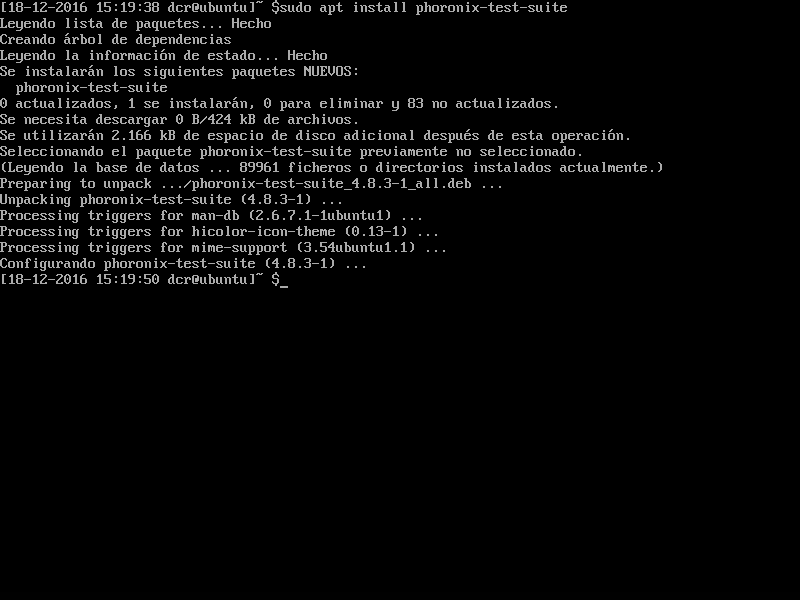
\includegraphics[scale=0.4]{phoronixInstall.png}
	\caption{Realizamos la instalación de \textit{Phoronix Suite} con \textit{apt} en Ubuntu Server 14.04.}
\end{figure}
 \verb|phoronix-test-suite| consultamos la lista de benchmarks disponibles ejecutando la orden \verb|phoronix-test-suite list-available-tests|. Como hay una lista muy grande utilizo la herramienta \textit{``grep''} para filtrar algún test que me interese, en concreto estoy interesado en buscar alguno de memoria.

\begin{figure}[H]
	\centering
	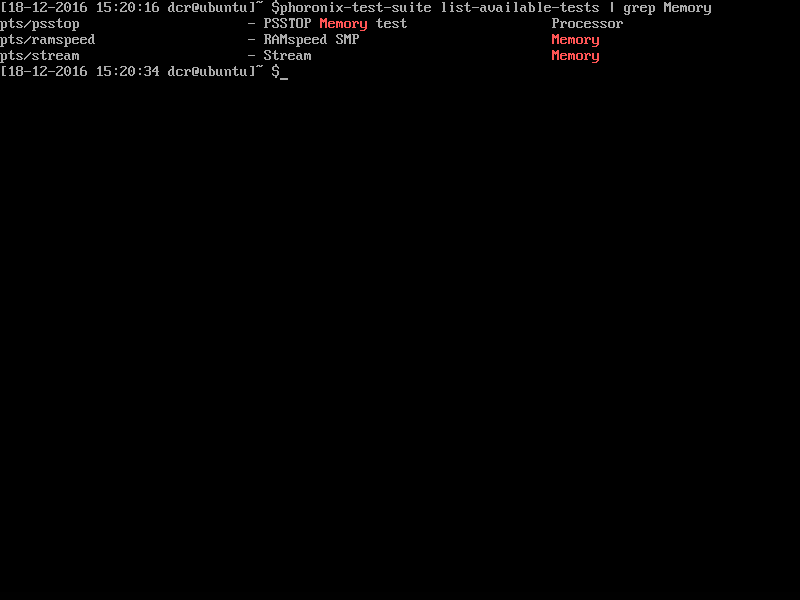
\includegraphics[scale=0.4]{phoronixMemory.png}
	\caption{Listado de test de memoria en \textit{Phoronix Suite}.}
\end{figure}

En mi caso, he decidido que voy a realizar el test denominado \textit{pts/ramspeed}. Para ejecutar e instalar el benchmark uso el comando \verb|phoronix-test-suite benchmark <nombre-test>|. \cite{c1}

\begin{figure}[H]
	\centering
	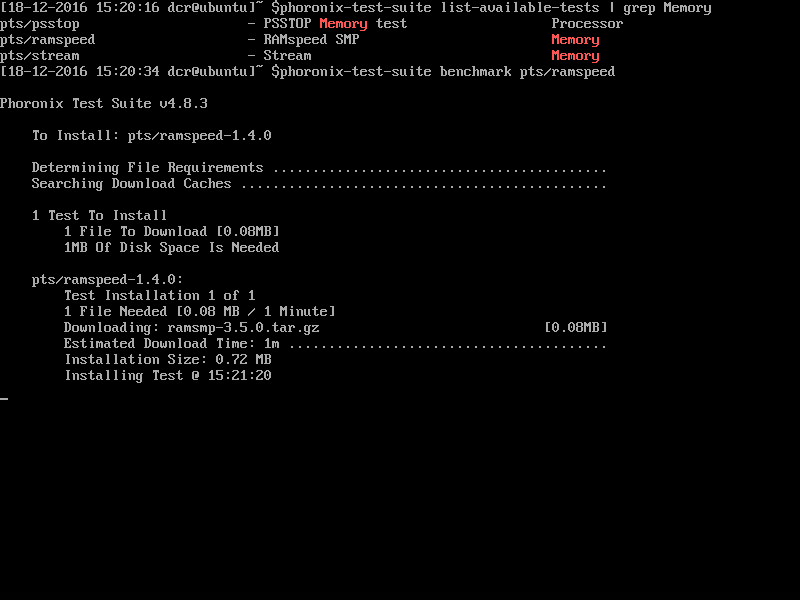
\includegraphics[scale=0.4]{testDownload.png}
	\caption{Como es la primera vez que se realiza el test, se inicia la descarga del mismo.}
\end{figure}

\begin{figure}[H]
	\centering
	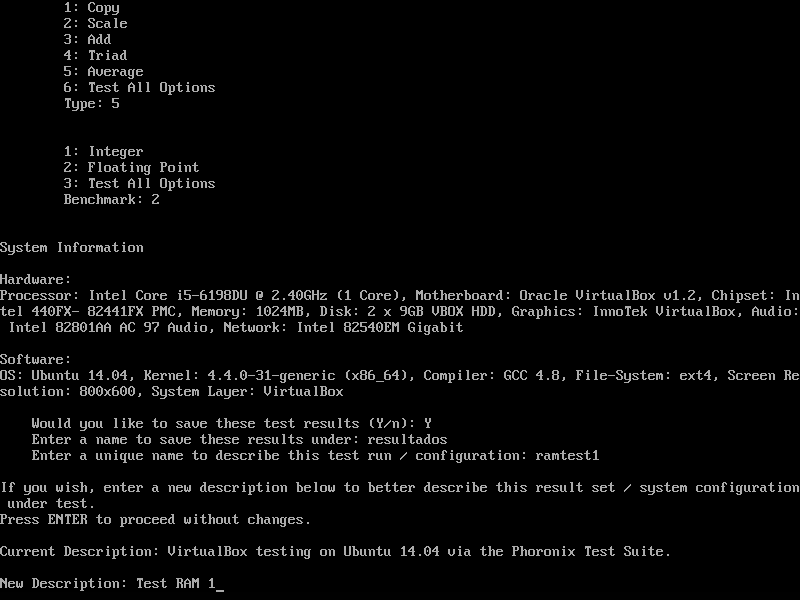
\includegraphics[scale=0.4]{testExec.png}
	\caption{Escojo una opción del test, en mi caso, velocidad media \textit{(5. Average)}. y con datos en coma flotante \textit{(2. Floating Point)}. Podemos observar la información del sistema y escoger el nombre de los datos a guardar.}
\end{figure}

Tras aproximadamente los 6 minutos indicados como tiempo estimado obteniendo de media \textbf{8486.04 MB/s}. 

Además, puesto que, como podemos observar, he escogido que los resultados sean compartidos en la web, podemos acceder desde Internet a los resultados del test (en caso de no compartirlo, dichos resultados también son guardados en la carpeta \linebreak \verb|.phoronix-test-suite/test-results/<nombre-a-guardar-test>| situada en la carpeta personal).

\begin{figure}[H]
	\centering
	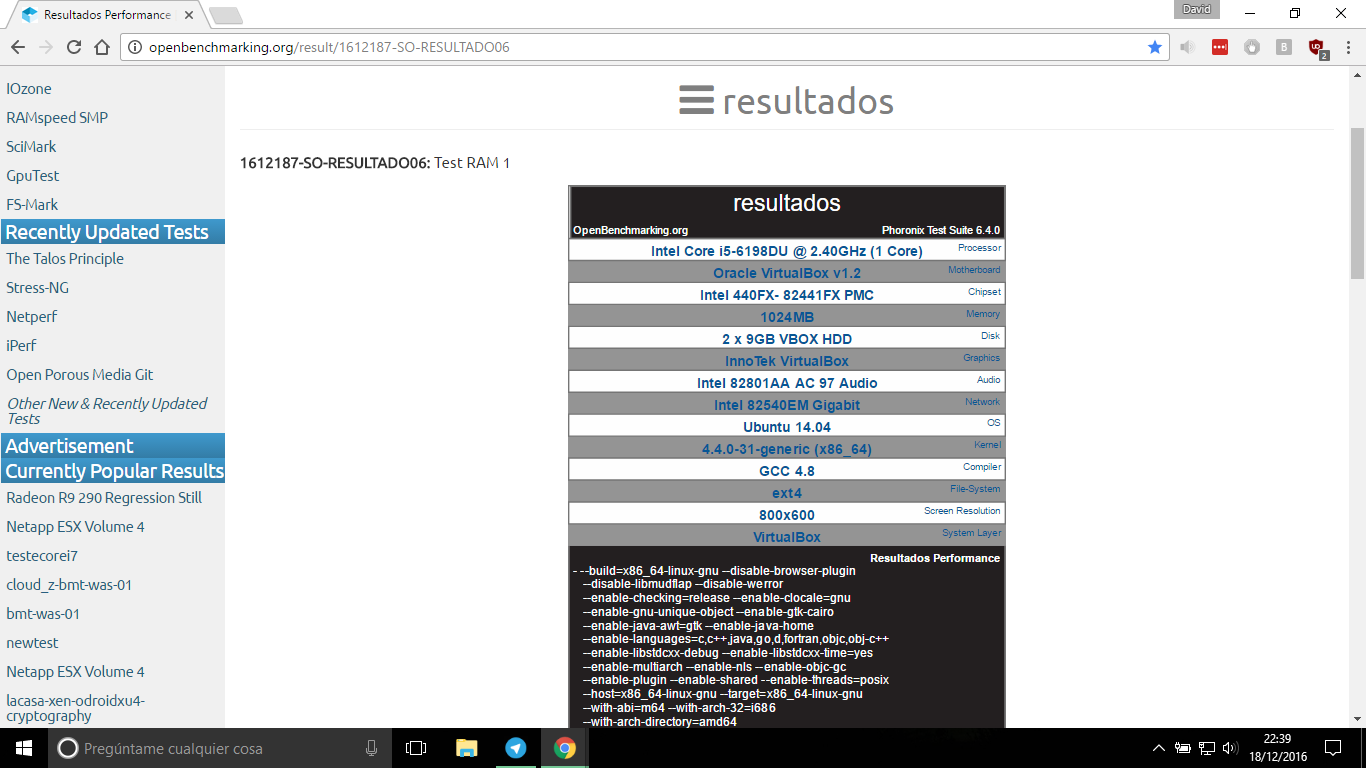
\includegraphics[scale=0.4]{phoronixResult.png}
	\caption{Información del PC que se ha usado para el benchmark.}
\end{figure}

\begin{figure}[H]
	\centering
	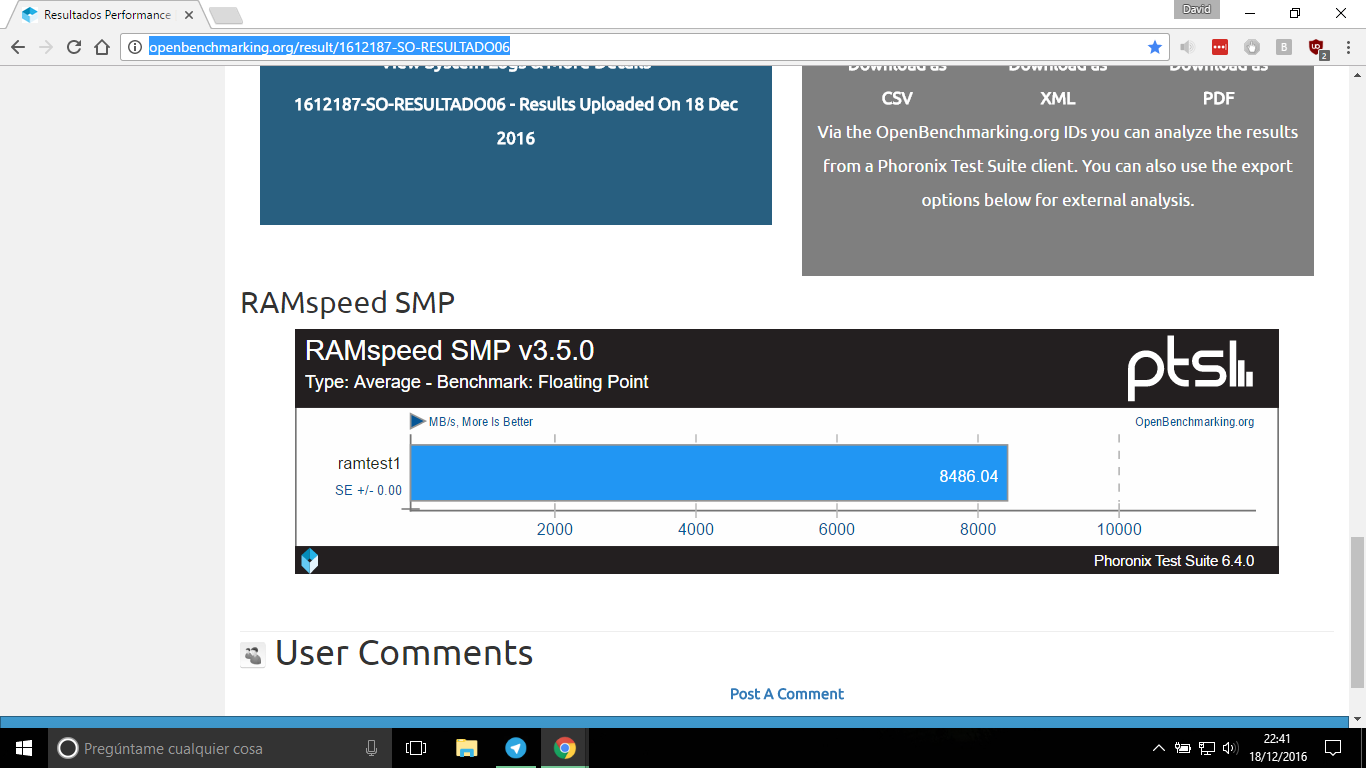
\includegraphics[scale=0.4]{phoronixResult2.png}
	\caption{Información de los resultados del benchmark.}
\end{figure}

Tras ejecutar el test podemos observar que aunque la máquina virtual sólo tiene asignada 1 GiB de memoria RAM la velocidad por segundo que es capaz de alcanzar es superior a los 8 GiB por segundo de los que dispone la máquina anfitriona.

%----------------------------------------------------------------------------------------
%	Cuestión 2
%----------------------------------------------------------------------------------------
\section{De los parámetros que le podemos pasar al comando ab. ¿Qué signficia -c 5? ¿y -n 100? Monitorice la ejecución de ab contra alguna máquina (cualquiera), ¿cuántas ``tareas'' crea ab en el cliente?}

La opción -c \cite{c2} nos permite indicar el nivel de concurrencia a usar, es decir, ``el número de peticiones que se deben realizar al mismo tiempo'' (si no lo indicamos por defecto es 1). \linebreak

La opción -n indica el número de peticiones que se han de realizar (si no lo indicamos por defecto es 1).

Tras ejecutar ab desde la máquina virtual con CentOS 7 sobre la página principal del servidor web en Ubuntu Server 14.04 podemos observar que se crea una única hebra de ab en el cliente, aunque en el servidor, con el objetivo de responder las peticiones, podemos observar hasta 75 hebras concurrentes, tal y como apreciamos en la siguiente captura.

\begin{figure}[H]
	\centering
	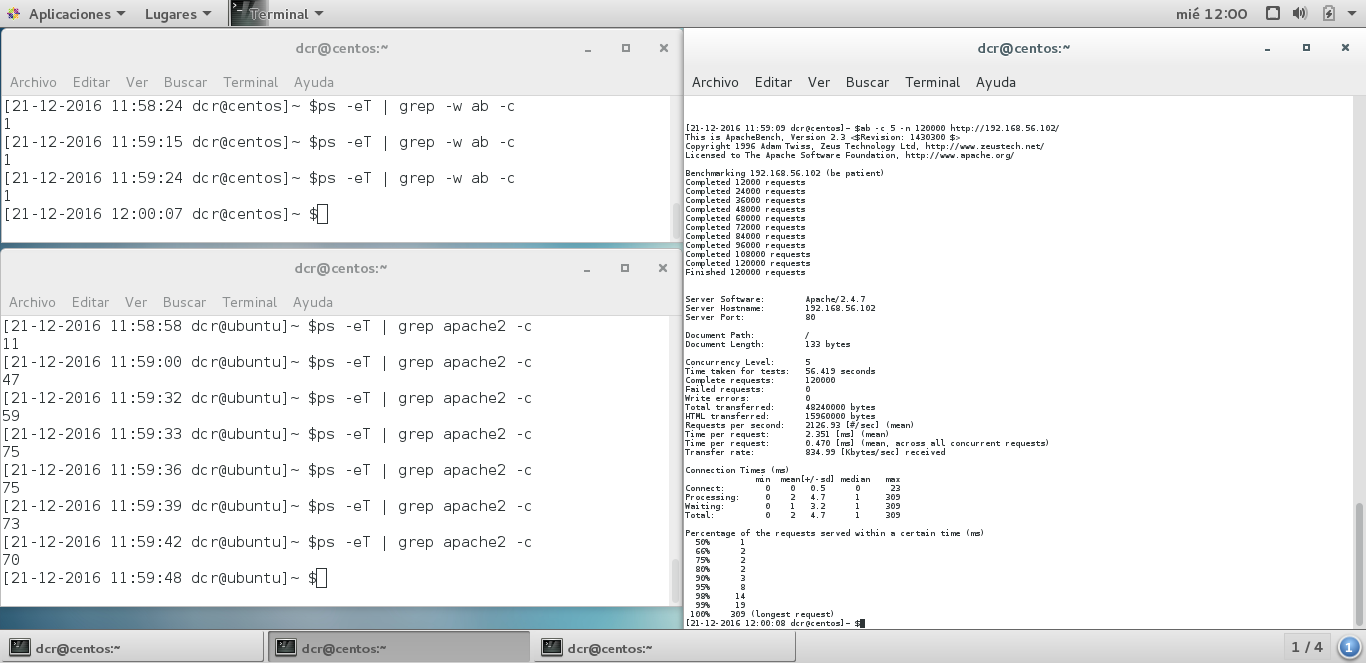
\includegraphics[scale=0.4]{ejer2.png}
	\caption{A la izquierda, en la parte superior, comprobamos el número de hebras de \textit{ab}. En la parte inferior, comprobamos el número de hebras de \textit{apache2}. A la derecha la ejecución de \textit{ab}.}
\end{figure}

%----------------------------------------------------------------------------------------
%	Cuestión 3
%----------------------------------------------------------------------------------------
\section{Ejecute ab contra a las tres máquinas virtuales (desde el SO anfitrión a las máquina virtuales de la red local) una a una (arrancadas por separado).¿Cuál es la que proporciona mejores resultados? Muestre y coméntelos. (Use como máquina de referencia Ubuntu Server para la comparativa).}
Todas las pruebas han sido realizadas con 120000 peticiones y un nivel de concurrencia de 5. Para que las pruebas sean válidas utilizamos el siguiente código HTML (Hypertext Markup Language).

\begin{verbatim}
<html>
<head><title>TEST AB</title></head>
<body>Esto es una página de prueba para hacer el benchmarking web de ISE.</body>
</html>
\end{verbatim}
\begin{figure}[H]
	\centering
	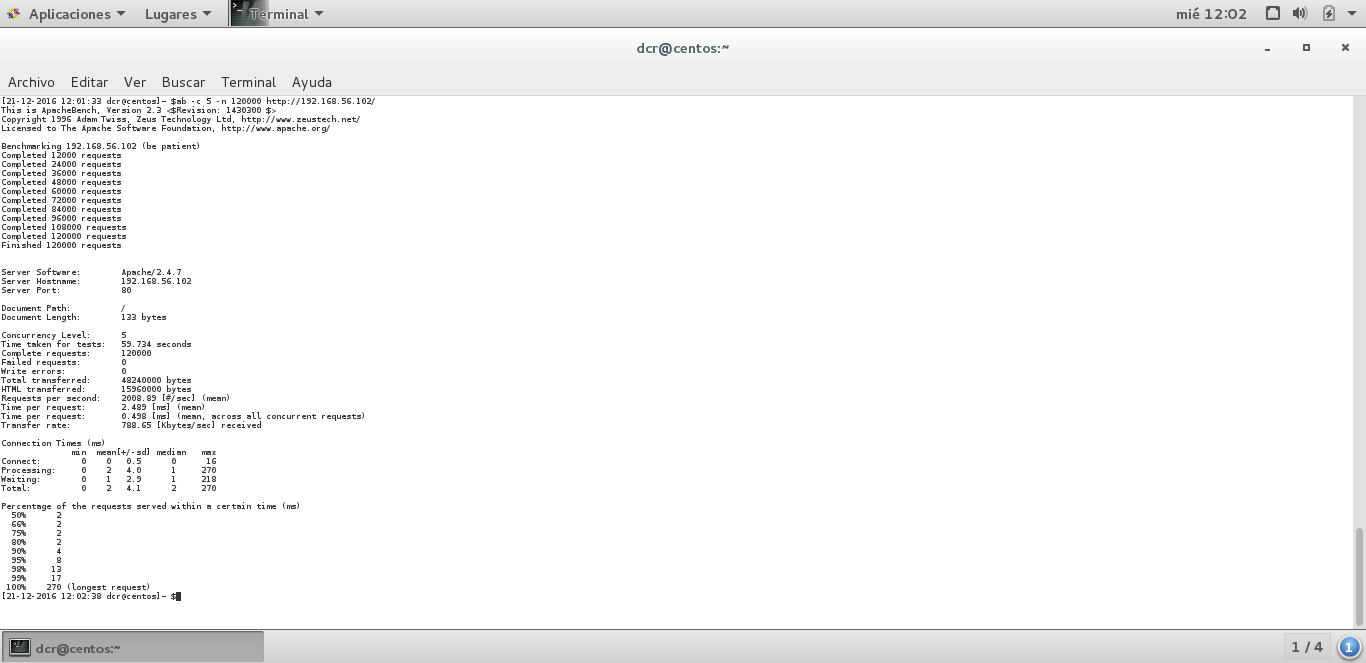
\includegraphics[scale=0.6]{abUbuntu.png}
	\caption{Ejecución de \textit{ab} desde CentOS contra el servidor web de Ubuntu Server.}
\end{figure}

\begin{figure}[H]
	\centering
	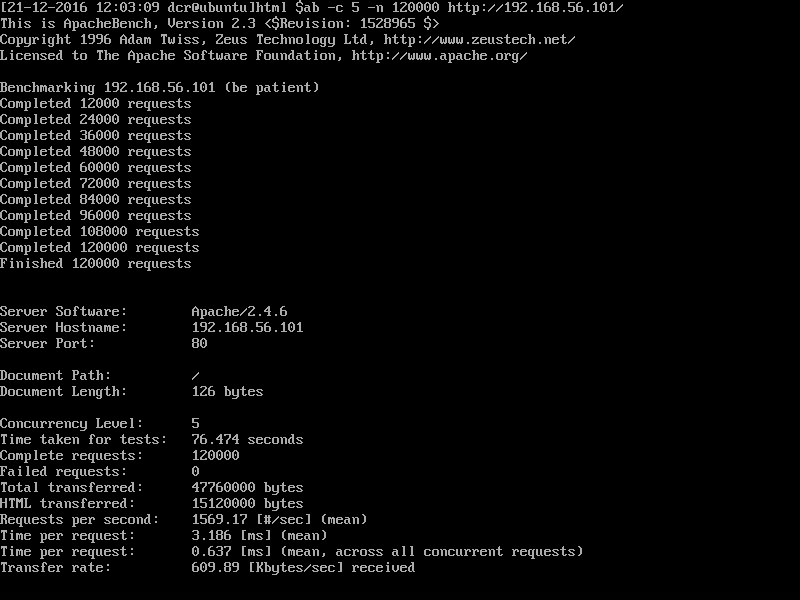
\includegraphics[scale=0.6]{abCentOS1.png}
	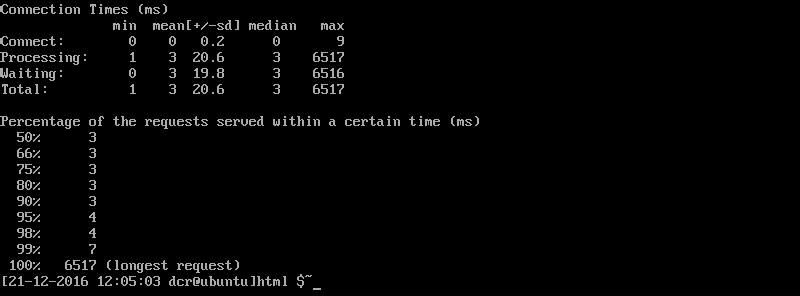
\includegraphics[scale=0.6]{abCentOS2.png}
	\caption{Ejecución de \textit{ab} desde Ubuntu Server 14.04 contra el servidor web de CentOS.}
\end{figure}

\begin{figure}[H]
	\centering
	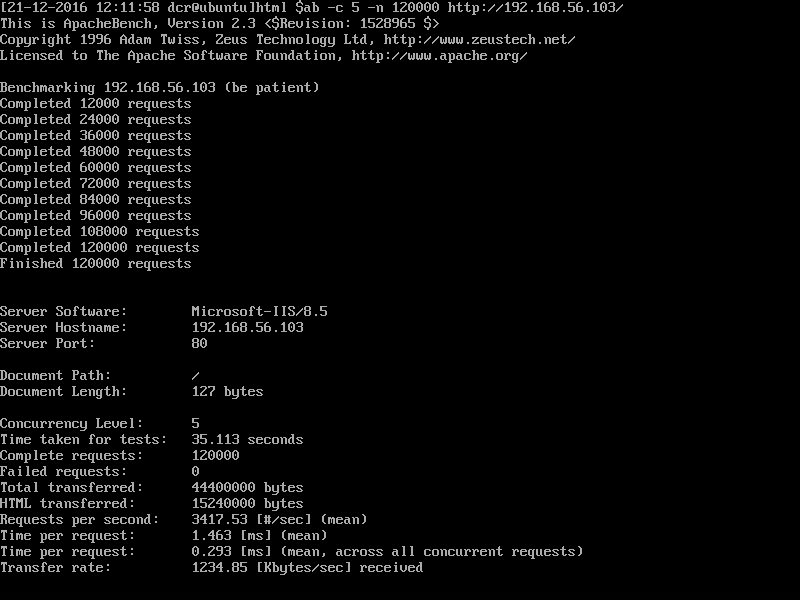
\includegraphics[scale=0.6]{abWindows1.png}
	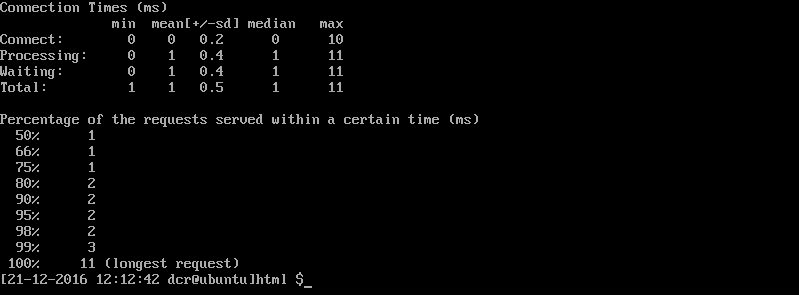
\includegraphics[scale=0.6]{abWindows2.png}
	\caption{Ejecución de \textit{ab} desde Ubuntu Server 14.04 contra el servidor web de Windows Server.}
\end{figure}

Para comparar todos los servidores utilizamos la métrica de peticiones por segundo.
\begin{table}[H]
	\centering
	\label{my-label}
	\begin{tabular}{|c|c|c|}
		\hline
		\textbf{Ubuntu Server 14.04} & \textbf{CentOS 7}        & \textbf{Windows Server 2012 R2} \\ \hline
		2008,89 \#/segundo    & 1569,17 \#/segundo  & 3417,53 \#/segundo        \\ \hline
	\end{tabular}
	\caption{Comparación de peticiones por segundo con ab para cada sistema operativo.}
\end{table}

Podemos observar que con diferencia Windows Server ha ofrecido los mejores resultados y que el siguiente mejor ha sido Ubuntu Server y, por último, CentOS que tiene más overhead que la otra distribución de Linux, entre otros, por el consumo que tiene la interfaz gráfica del sistema operativo.
%----------------------------------------------------------------------------------------
%	Cuestión 4
%----------------------------------------------------------------------------------------
\section{Instale y siga el tutorial en http://jmeter.apache.org/usermanual/build-web-test-plan.html realizando capturas de pantalla y comentándolas. En vez de usar la web de meter, haga el experimento usando sus máquinas virtuales ¿coincide con los resultados de ab?}
Para instalarlo simplemente descargamos el zip y ejecutamos el archivo \textit{jmeter.bat} en la carpeta bin (es necesario tener instalado Java en el sistema).
Tras leer el tutorial, seguimos los siguientes pasos para preparar el test.

\begin{figure}[H]
	\centering
	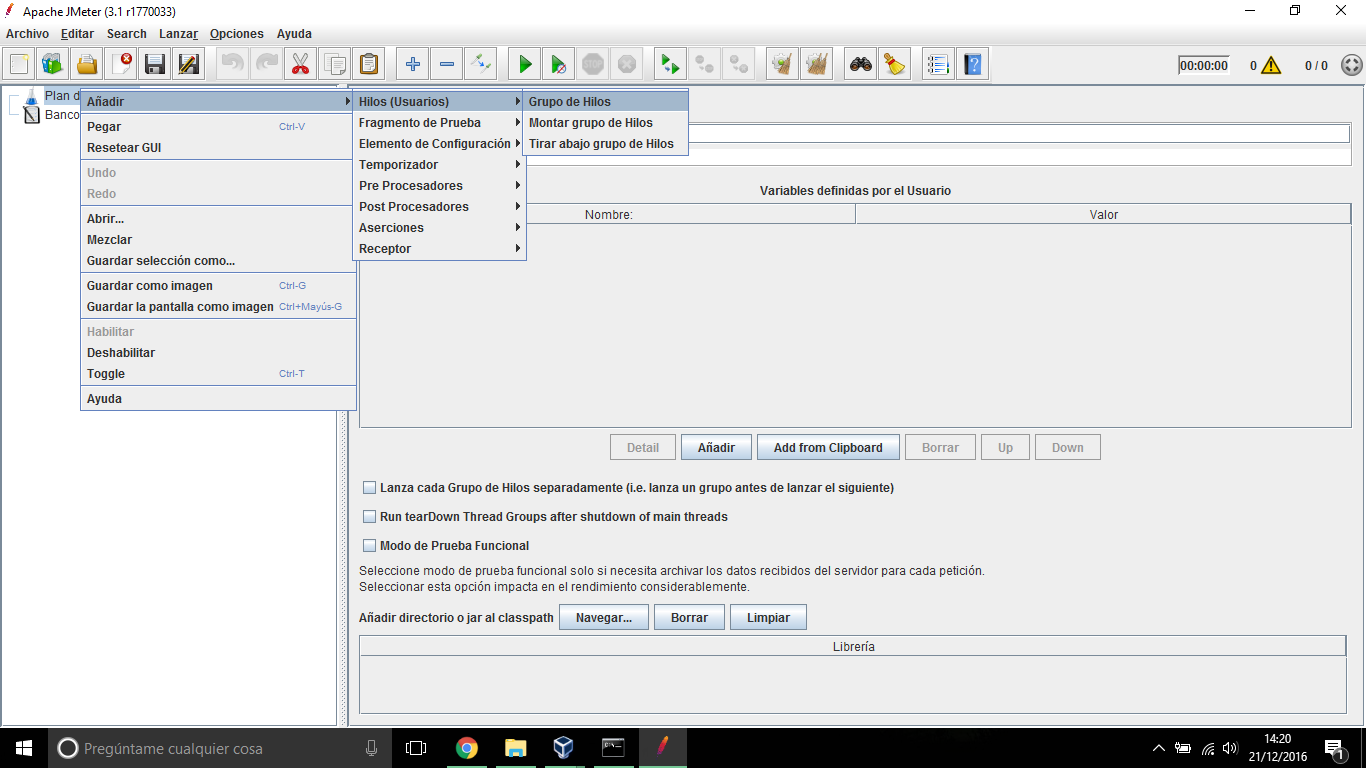
\includegraphics[scale=0.3]{jmeter1.png}
	\caption{Haciendo click derecho en el plan seleccionamos \textit{Hilos(Usuarios)} y marcamos \textit{Grupos de Hilos}.}
\end{figure}
\begin{figure}[H]
	\centering
	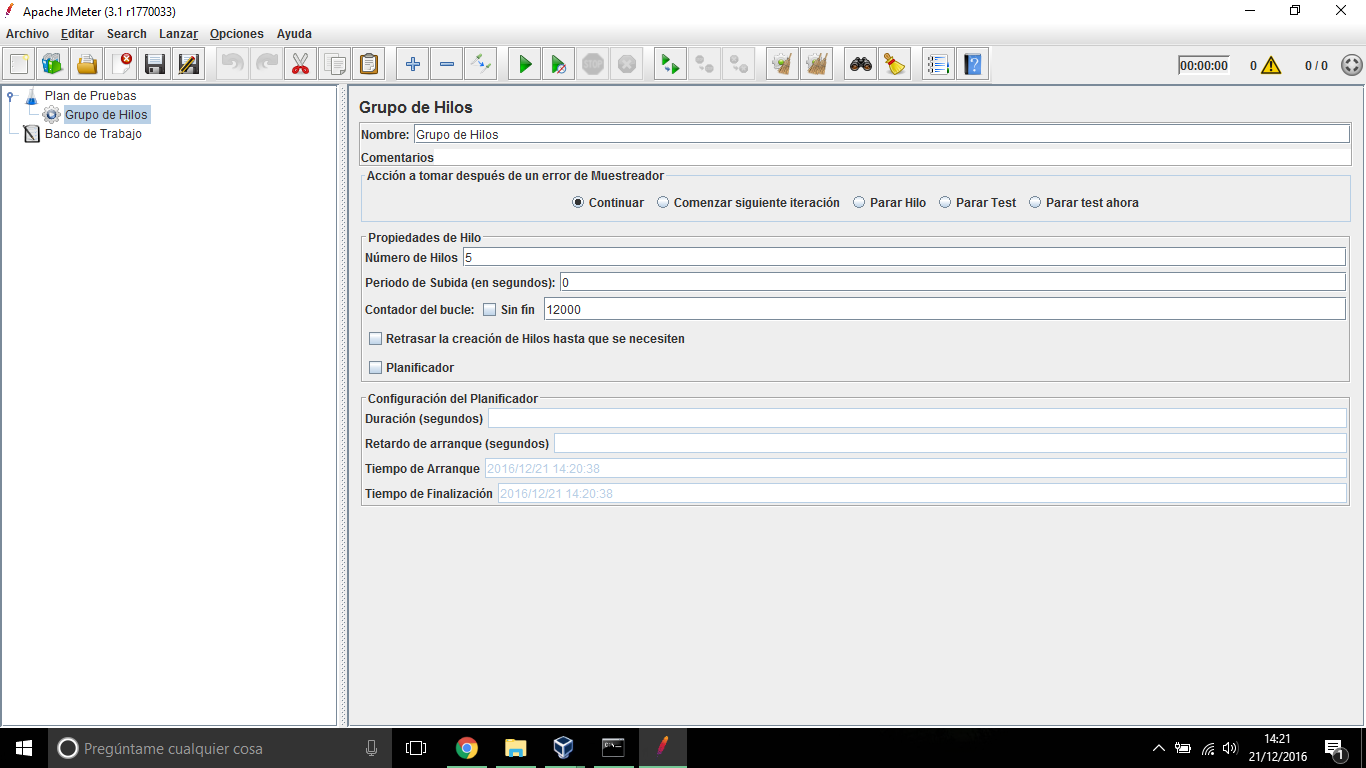
\includegraphics[scale=0.3]{jmeter2.png}
	\caption[Grupo de Hilos en Apache JMeter.]{Indicamos el número de hebras que vamos a usar en \textit{Número de Hilos} el tiempo en el que van entrando \textit{Periodo de Subida (en segundos)} que dejamos a 0 (para que se inicien todos a la vez) y en el \textit{Contador de bucle} ponemos el número de peticiones que ha de hacer cada hebra (al final lo dejé a 24000) para obtener una cantidad de muestras similar a las de ab.}
\end{figure}
\begin{figure}[H]
	\centering
	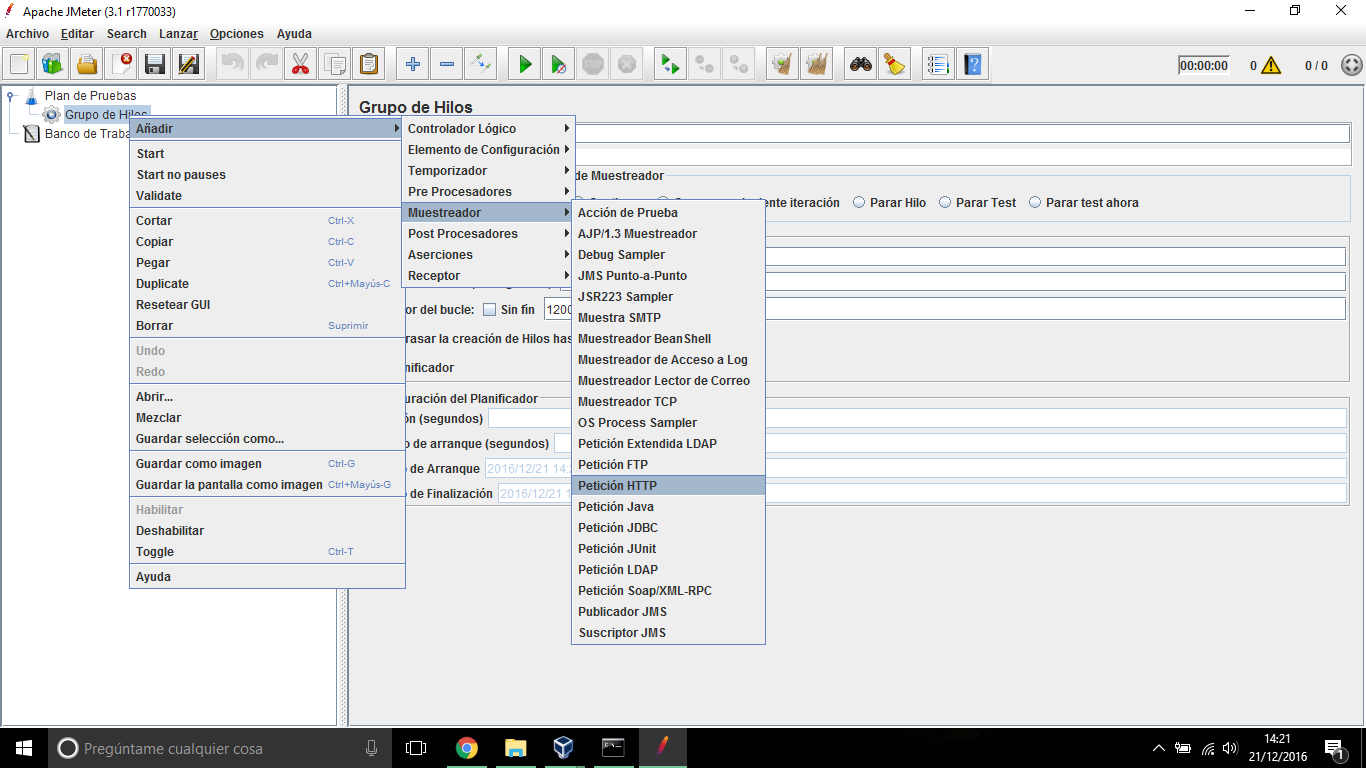
\includegraphics[scale=0.3]{jmeter3.png}
	\caption{Haciendo click derecho en el \textit{Grupo de Hilos} escogemos \textit{Añadir -> Muestreador -> Petición HTTP}.}
\end{figure}
\begin{figure}[H]
	\centering
	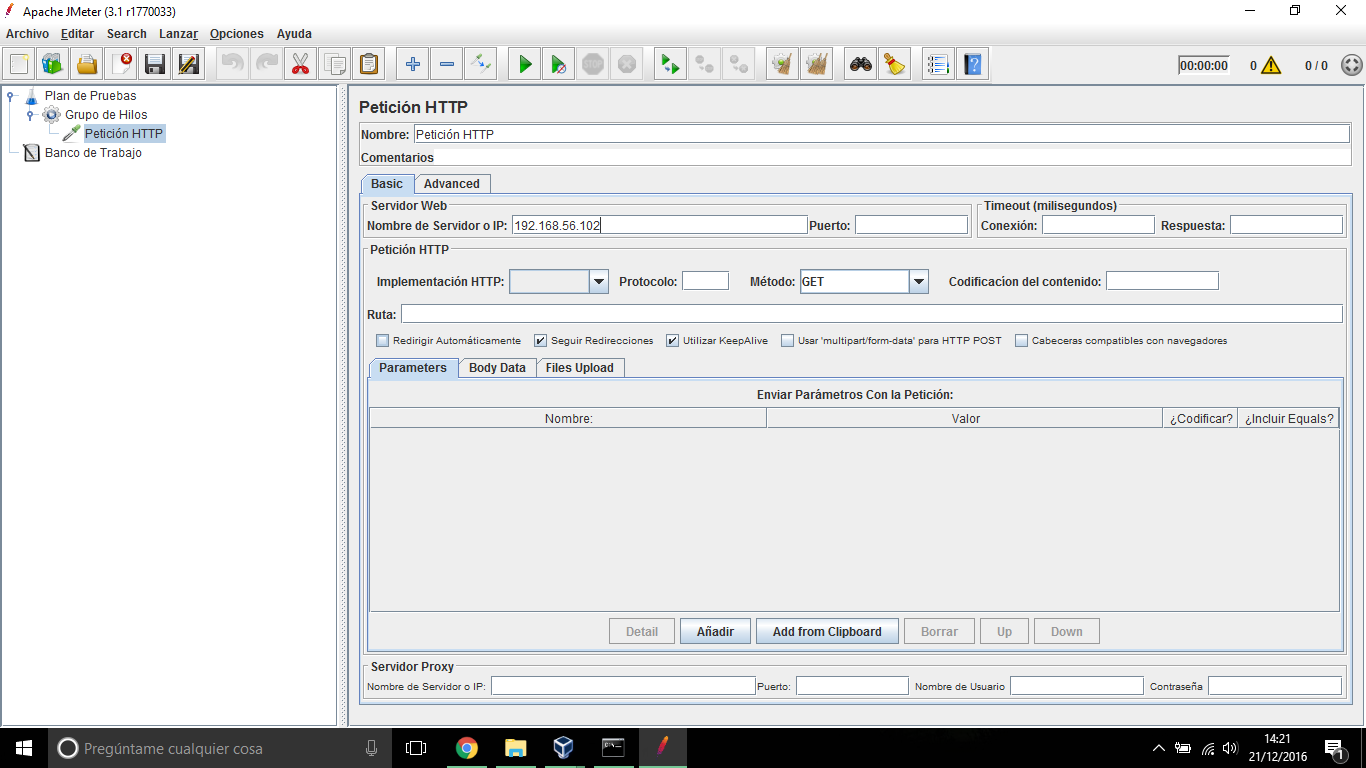
\includegraphics[scale=0.3]{jmeter4.png}
	\caption{En el campo de \textit{Nombre de Servidor o IP.} seleccionamos la IP del servidor al que vamos a hacer el benchmark.}
\end{figure}
\begin{figure}[H]
	\centering
	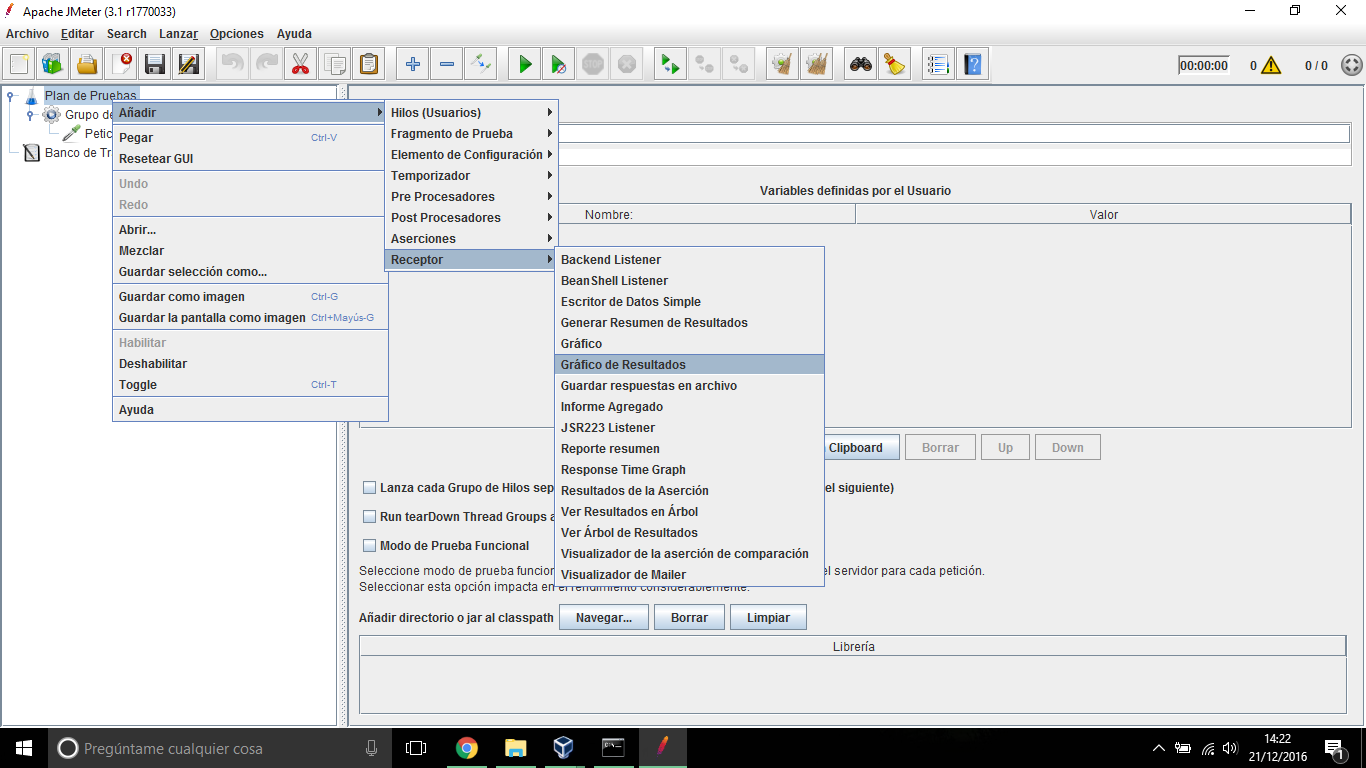
\includegraphics[scale=0.3]{jmeter5.png}
	\caption{Hacemos click derecho en el \textit{Plan de Pruebas} escogemos \textit{Añadir -> Receptor -> Gráfico de Resultados}.}
\end{figure}
\begin{figure}[H]
	\centering
	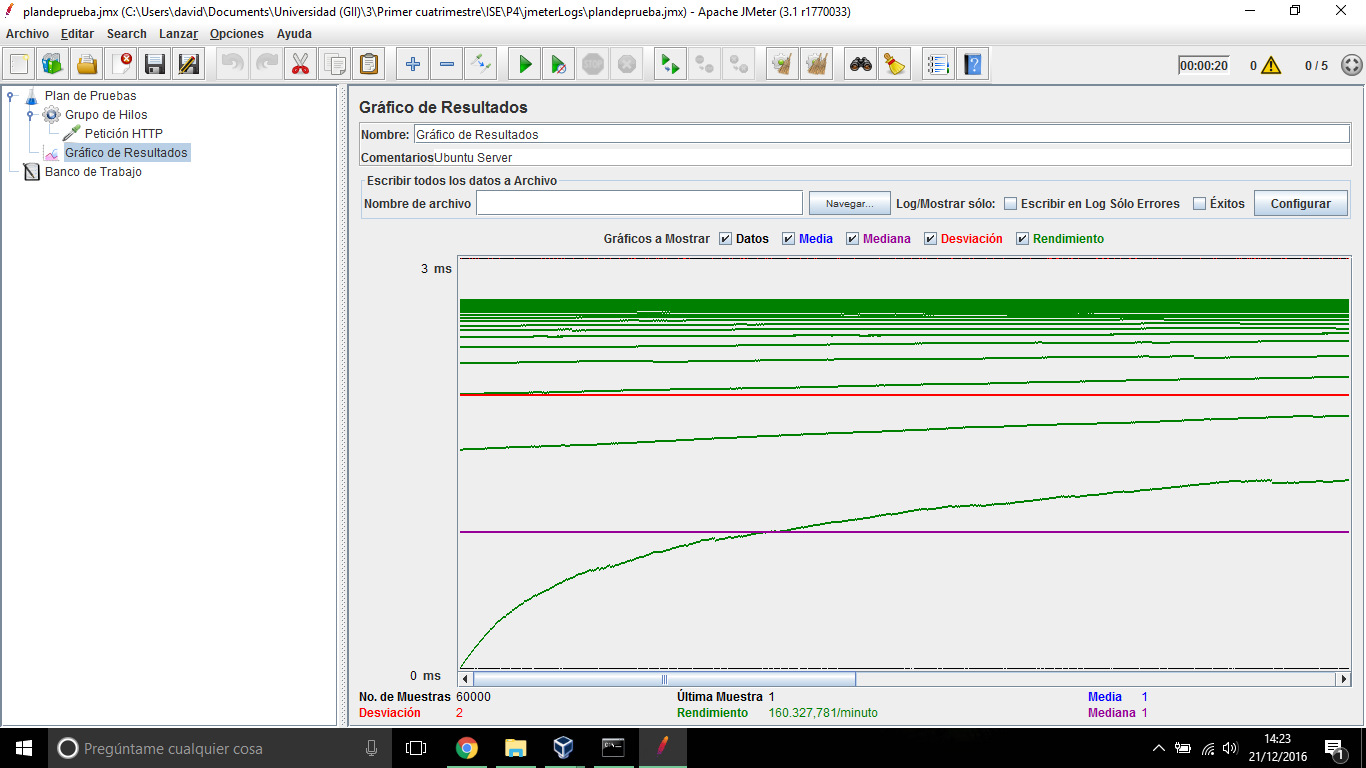
\includegraphics[scale=0.3]{jmeter6.png}
	\caption{Tras pulsar en el botón de ejecutar y esperar obtenemos un gráfico como este.}
\end{figure}

Como podemos observar, en este ejemplo he realizado el benchmark sobre Ubuntu Server 14.04 indicando su dirección IP (192.168.56.102) y observamos un \textit{Rendimiento} de 160.327,781/minuto. Para que las muestras sean más o menos similares aumentamos el contador del bucle a 24000. Tras realizarlo sobre las 3 máquinas obtenemos los siguientes resultados:

\begin{figure}[H]
	\centering
	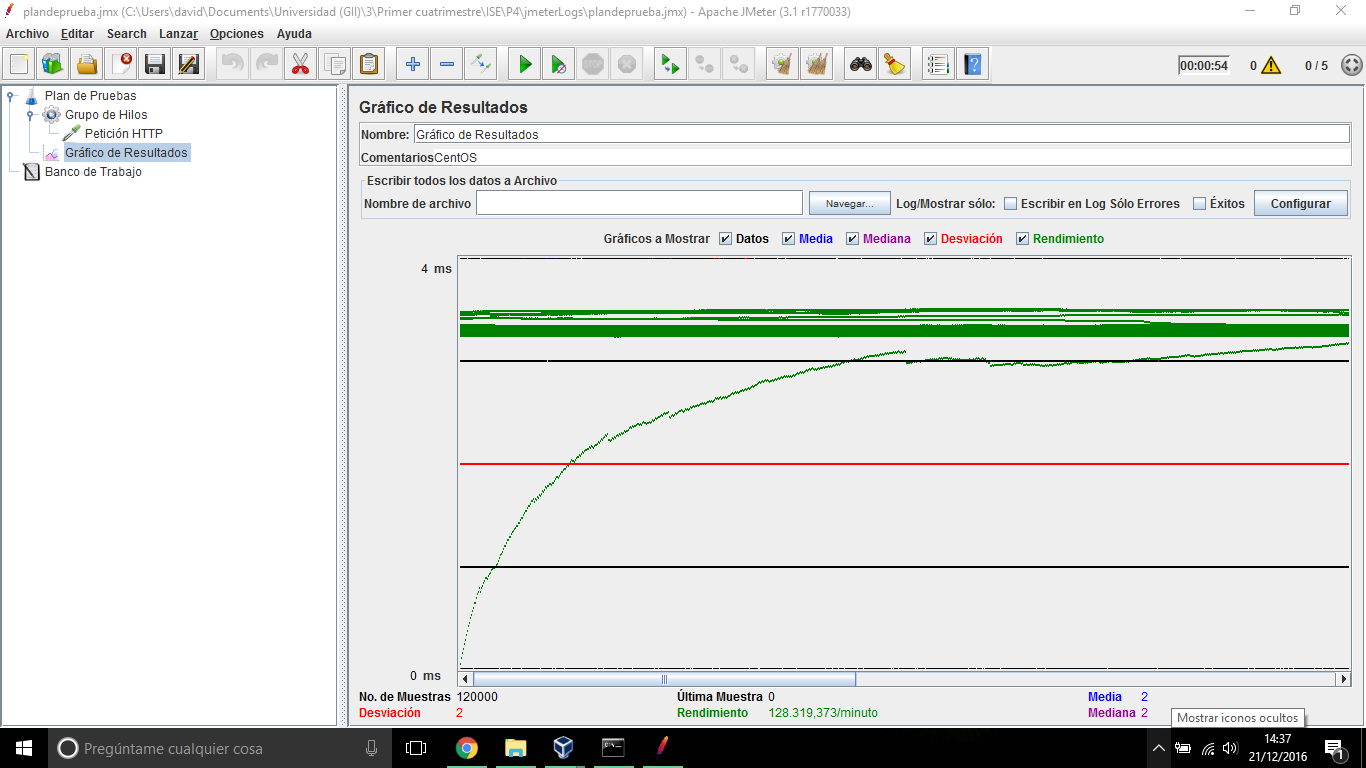
\includegraphics[scale=0.3]{jmeterCentOS.png}
	\caption{Resultados de Apache JMeter tras ejecutarlo desde el anfitrión contra el servidor web en CentOS.}
\end{figure}

\begin{figure}[H]
	\centering
	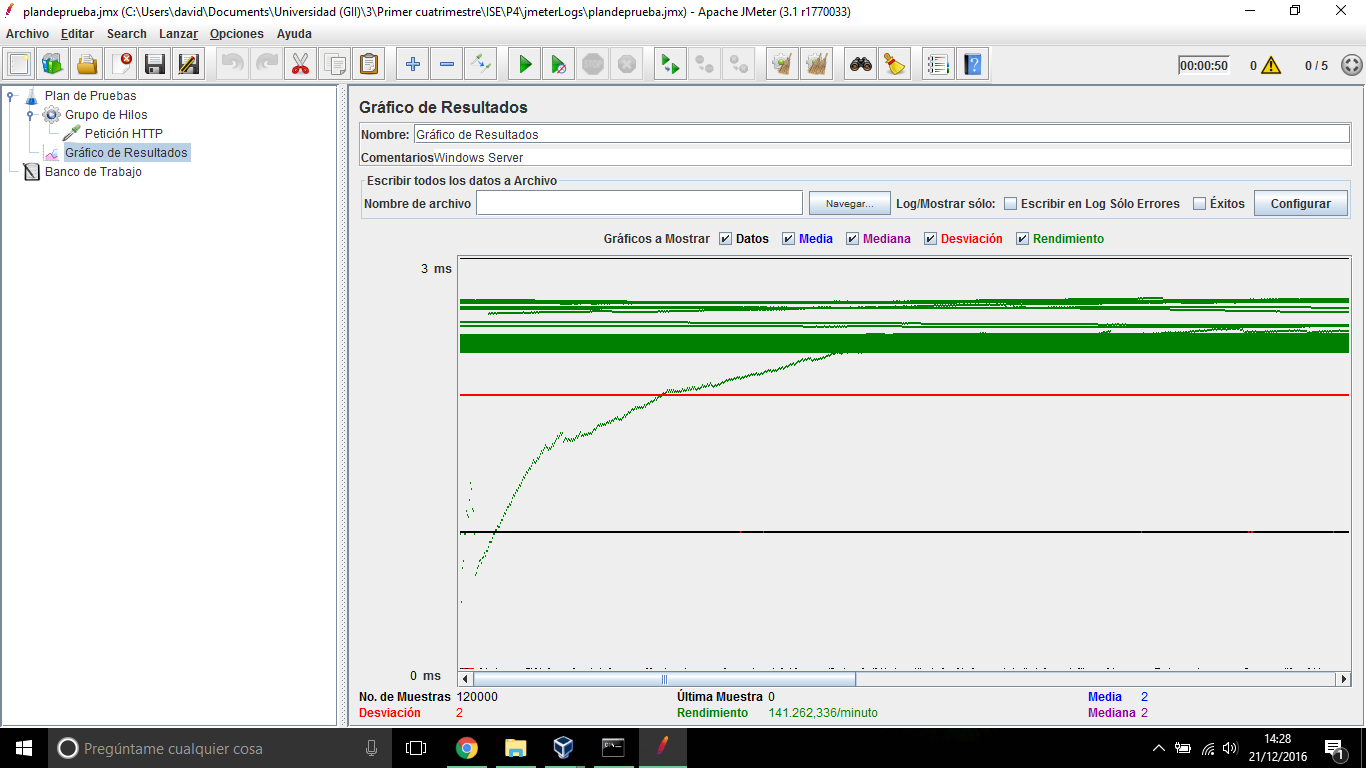
\includegraphics[scale=0.3]{jmeterWindows.png}
	\caption{Resultados de Apache JMeter tras ejecutarlo desde el anfitrión contra el servidor web en Windows Server.}
\end{figure}

\begin{figure}[H]
	\centering
	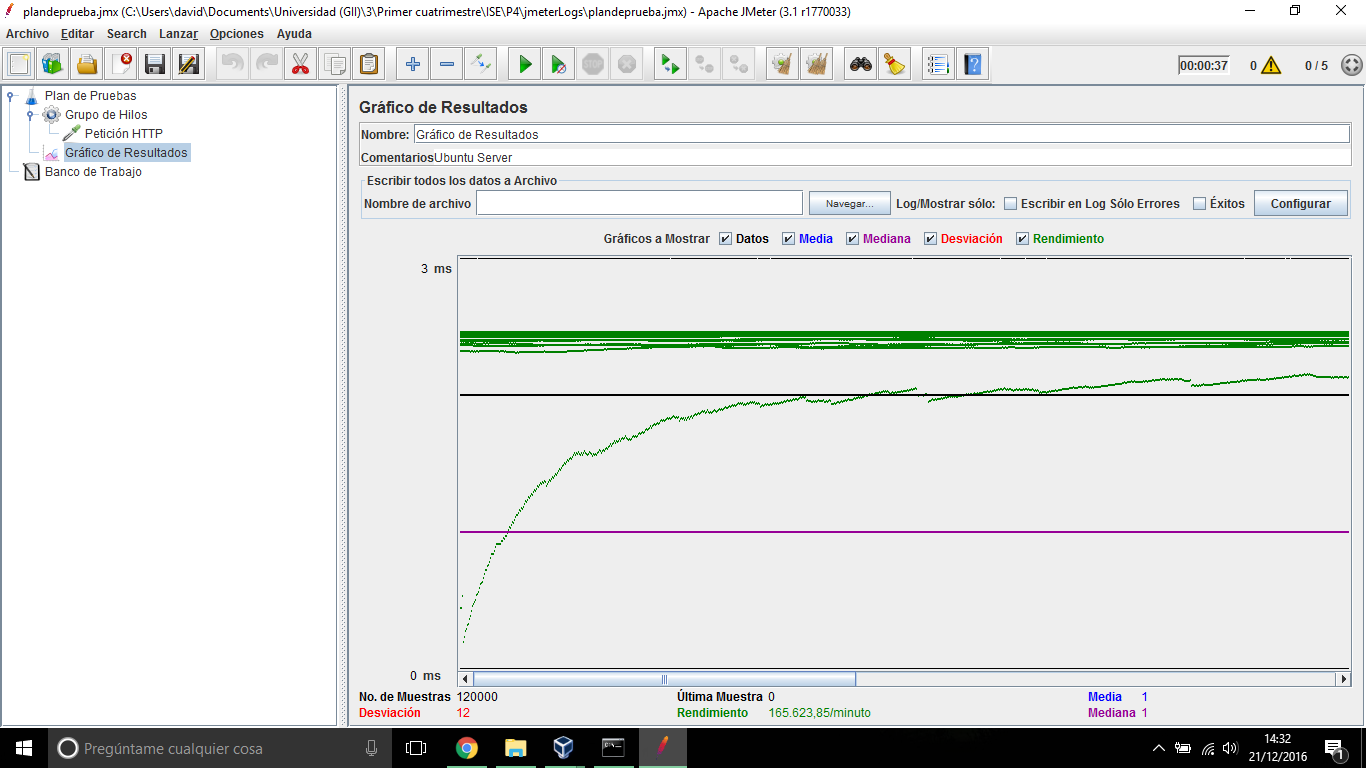
\includegraphics[scale=0.3]{jmeterUbuntu.png}
	\caption{Resultados de Apache JMeter tras ejecutarlo desde el anfitrión contra el servidor web en Ubuntu Server.}
\end{figure}

Tras pasar las peticiones por segundo a peticiones por minuto de los resultados de \textit{ab} y el rendimiento de \textit{Apache JMeter} (que se mide en peticiones por minuto también).

\begin{table}[H]
	\centering
	\label{my-label}
	\begin{tabular}{c|c|c|c|}
		\cline{2-4}
		\multicolumn{1}{l|}{}                 & \textbf{Ubuntu Server 14.04}              & \textbf{CentOS 7}                          & \textbf{Windows Server 2012 R2} \\ \hline
		\multicolumn{1}{|c|}{\textbf{ab}}     & 120.533,4 \#/minuto                       & 94.150,20 \#/minuto                        & 205.051,80 \#/minuto            \\ \hline
		\multicolumn{1}{|c|}{\textbf{JMeter}} & \multicolumn{1}{l|}{165.623,85 \#/minuto} & \multicolumn{1}{l|}{128.319,373 \#/minuto} & 141.266,63 \#/minuto            \\ \hline
	\end{tabular}
	\caption{Comparativa de servidores web con ab y JMeter.}
\end{table}

Podemos ver que con este test se determina que el más lento de todos es CentOS pero en este caso Ubuntu Server es más rápido que Windows Server. Es posible que el hecho de que al usar ab necesitase tener abierta otra máquina virtual añadiése algún overhead a la hora de realizar los benchmarks.

%----------------------------------------------------------------------------------------
%	Cuestión 5
%----------------------------------------------------------------------------------------
\section{Programe un benchmark usando el lenguaje que desee.}
El objetivo del benchmark es medir la ejecución con múltiples hebras de una CPU, para ello vamos a, en cada repetición, crear un grupo de hebras ejecutar el mismo algoritmos en todas las hebras, unirlas y medir el tiempo transcurrido. La métrica a usar será el tiempo de ejecución (medido en segundos) medio de todos los intervalos. Como el benchmark lo voy a programar con C++11 utilizaré la librería \textit{thread} \cite{c5a} para crear hebras concurrentes y la librería \textit{chrono} \cite{c5b} para realizar mediciones de tiempo lo más precisas posibles. Además, el programa permitirá pasar como parámetro si usar enteros o números en coma flotante, el número de hebras, las repeticiones, y si queremos usar un algoritmo cuadrático (ordenación por burbuja), ordenación n log n con std::sort o un algoritmo lineal que realiza operaciones matemáticas sobre cada número. Es importante que se compile sin optimizaciones el código para obtener resultados válidos. El código del benchmark sería el siguiente:

\begin{verbatim}
#include <algorithm>
#include <chrono>
#include <iostream>
#include <stdexcept>
#include <random>
#include <thread>
#include <vector>

// Generamos números en coma flotante aleatorios (No cuenta para el tiempo del benchmark).
void genereteRandom(auto& v, unsigned size) {
std::random_device rd;
std::mt19937 mt(rd());
std::uniform_real_distribution<double> dist;

v.resize(size);
for (auto& d: v)
d = dist(mt);
}

// Opción para complejidad cuadrática
void sortBubble(auto& v) {
for (auto i =0u; i < v.size(); ++i)
for (auto j = 0u; j < v.size() - i; ++j)
if (v[j] > v[j+1])
std::swap(v[j], v[j+1]);
}

void sortBubbleInt(std::vector<int>& v) { std::vector<int> a;
std::copy(std::begin(v),std::end(v),std::back_inserter(a));
sortBubble(a); }
void sortBubbleFloat(std::vector<double>& v) { std::vector<double> a;
std::copy(std::begin(v),std::end(v),std::back_inserter(a));
sortBubble(a); }

// Opción para complejidad O(n log n)
void sortLog(auto v) {
std::sort(std::begin(v), std::end(v));
}

void sortLogInt(const std::vector<int>& v) { std::vector<int> a;
std::copy(std::begin(v),std::end(v),std::back_inserter(a));
sortLog(a); }
void sortLogFloat(const std::vector<double>& v) { std::vector<double> a;
std::copy(std::begin(v),std::end(v),std::back_inserter(a));
sortLog(a); }

// Opción para complejidad O(n)
void linear(auto v) {
for (auto& d: v)
d = (d + 2) / std::sqrt(d);
}

void sortLinearInt(const std::vector<int>& v) { std::vector<int> a;
std::copy(std::begin(v),std::end(v),std::back_inserter(a));
linear(a); }
void sortLinearFloat(const std::vector<double>& v) { std::vector<double> a;
std::copy(std::begin(v),std::end(v),std::back_inserter(a));
linear(a); }

double averageTime(const std::vector<double>& times) {
double media = 0.0;
for (auto d: times)
media += d;
media /= times.size();

return media;
}

int main(int argc, char *argv[])
{
unsigned size, repetitions, concurrency, mode;
bool isFloat = false;
if (argc != 6) {
std::cerr << "Uso correcto: benchmark <tam_vector> <número de repeticiones> <float o int> <número de hebras>";
std::cerr << "<modo: 0 (cuadrático)|1(logarítmico)|2 lineal>\n";
return -1;
}
try {
size = std::stoi(argv[1]);
repetitions = std::stoi(argv[2]);
std::string myType = argv[3];

if (myType == "float")
isFloat = true;
else if (myType == "int")
isFloat = false;
else {
std::cerr << "Uso correcto: benchmark <tam_vector> <número de repeticiones> <float o int> <número de hebras>\n";
std::cerr << "<modo: 0 (cuadrático)|1(logarítmico)|2 lineal>\n";
std::cerr << "El tipo sólo puede ser float o int (en minúscula).\n";
return -1;
}
concurrency = std::stoi(argv[4]);

mode = std::stoi(argv[5]);
if (mode > 2) {
std::cerr << "Uso correcto: benchmark <tam_vector> <número de repeticiones> <float o int> <número de hebras>\n";
std::cerr << "<modo: 0 (cuadrático)|1(logarítmico)|2 lineal>\n";
return -1;
}

} catch (const std::invalid_argument&) {
std::cerr << "Uso correcto: benchmark <tam_vector> <número de repeticiones> <float o int> <número de hebras>\n";
return -1;
}

std::vector<std::thread> threads;
std::vector<double> repeatTimes;

std::vector<double> v;
std::vector<int> vi;

if (isFloat)
genereteRandom(v, size);
else
genereteRandom(vi, size);
for (auto i = 0u; i < repetitions; ++i) {
auto trAntes = std::chrono::high_resolution_clock::now();
for (auto j = 0u; j < concurrency; ++j)
if (isFloat) switch (mode) {
case 0: threads.emplace_back(&sortBubbleFloat,std::ref(v)); break;
case 1: threads.emplace_back(&sortLogFloat,std::ref(v)); break;
case 2: threads.emplace_back(&sortLinearFloat,std::ref(v)); break;
} else switch (mode) {
case 0: threads.emplace_back(sortBubbleInt,std::ref(vi)); break;
case 1: threads.emplace_back(sortLogInt,std::ref(vi)); break;
case 2: threads.emplace_back(sortLinearInt,std::ref(vi)); break;
}
for (auto& thread: threads)
thread.join();
auto trDespues = std::chrono::high_resolution_clock::now();
std::chrono::duration<double> time = trDespues - trAntes;
repeatTimes.push_back(time.count());
threads.clear();
}
double mediaConcurrente = averageTime(repeatTimes);

std::cout << "El tiempo medio de ejecución concurrente de una repetición con " <<
concurrency << " hebras es " << mediaConcurrente << " segundos.\n";

}
\end{verbatim}

\begin{figure}[H]
	\centering
	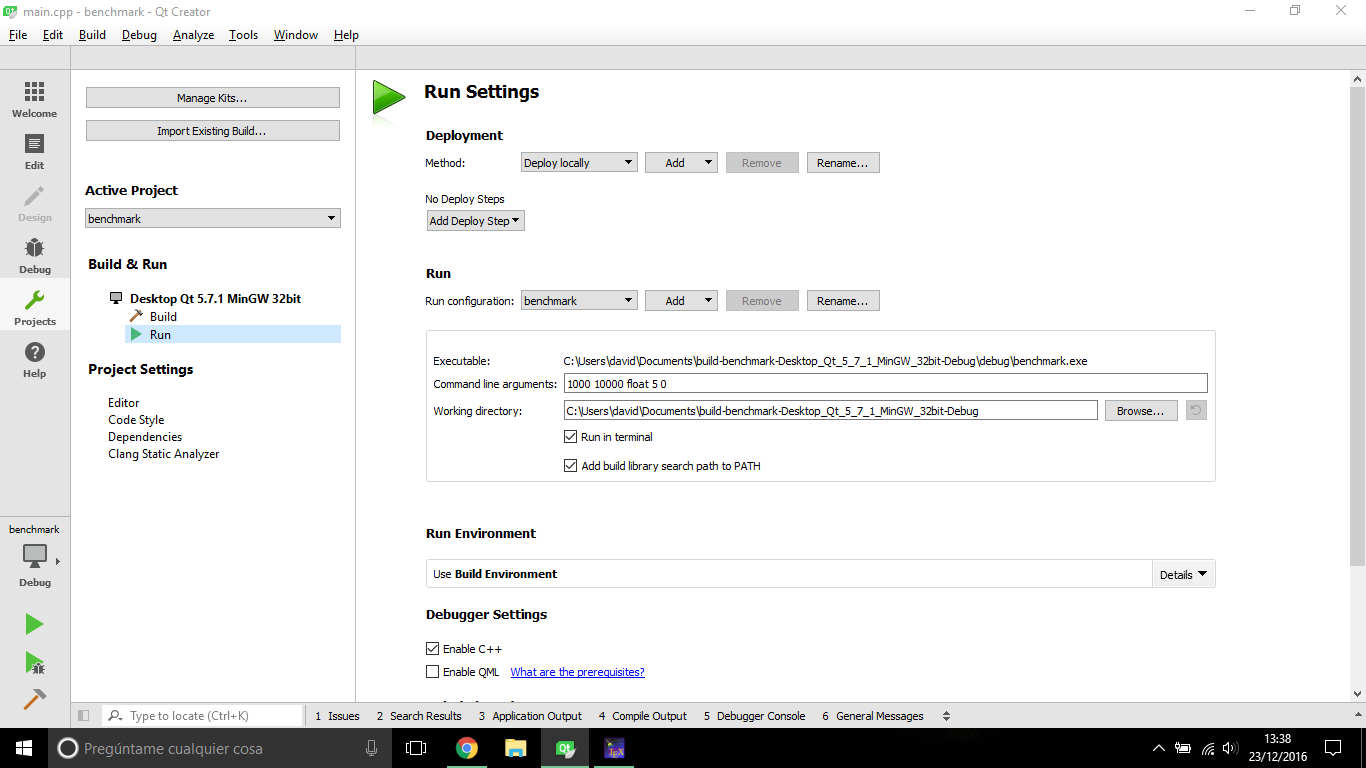
\includegraphics[scale=0.3]{parametros.png}
	\caption{Parámetros usados para ejecutar el benchmark propio.}
\end{figure}

Tras ejecutarlo en mi máquina anfitriona con los siguientes parámetros que se pueden ver en la figura
obtengo los resultados que se ven en la siguiente captura de pantalla.

\begin{figure}[H]
	\centering
	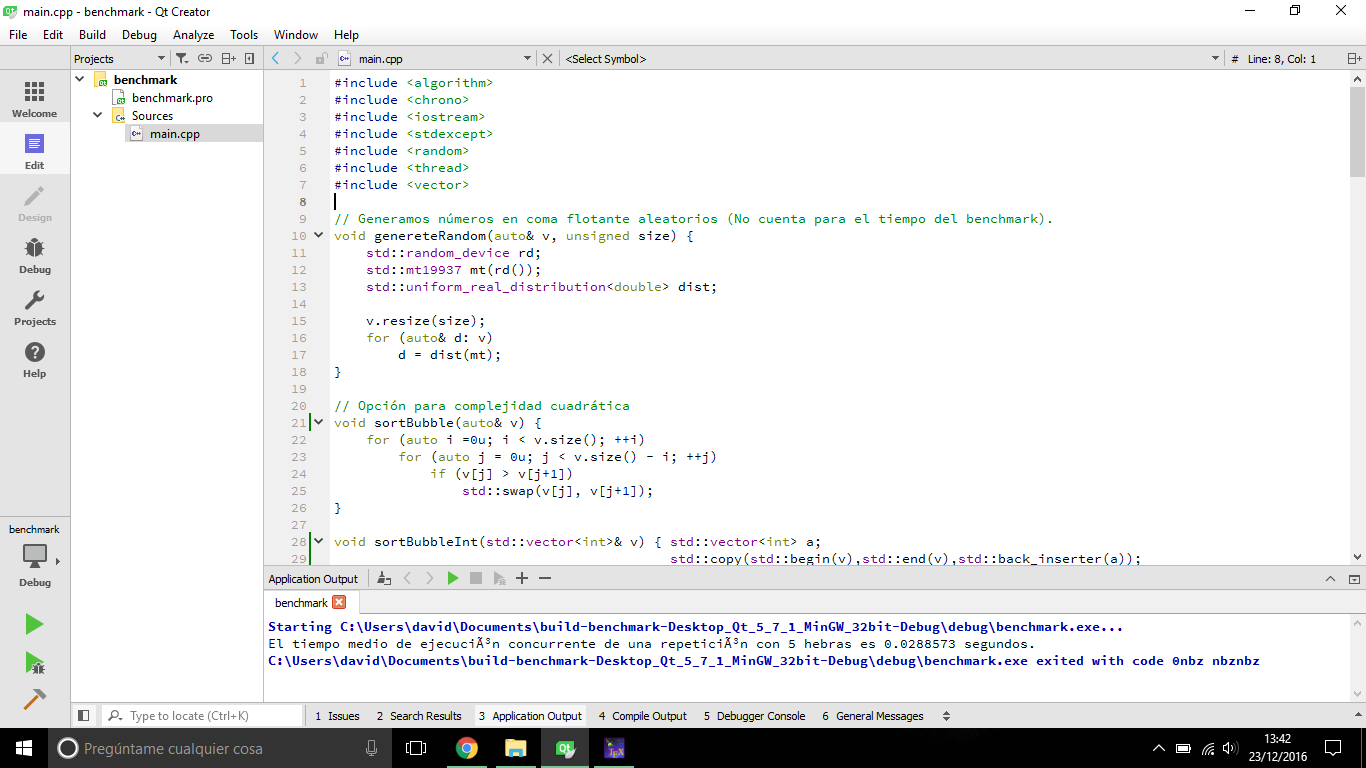
\includegraphics[scale=0.3]{ejecucion.png}
	\caption{En la parte inferior del IDE \textit{Qt Creator} vemos el resultado de ejecutar el benchmark con los parámetros previamente expuesto.}
\end{figure}

Como podemos observar el tiempo media que mi máquina anfitriona, con un Intel Core i5-6198DU tarda de media aproximadamente 0,03 segundos en que todas las hebras ejecuten una vez el algoritmo de ordenación burbuja sobre un vector de números en coma flotante de tamaño 1000. 
%----------------------------------------------------------------------------------------
%	Bibliografía
%----------------------------------------------------------------------------------------
\bibliography{citas} %archivo citas.bib que contiene las entradas 
\bibliographystyle{ieeetr} % hay varias formas de citar
\end{document}
